\scanpage{13}
resp. séparé resp... en type fini \unsure{resp.} séparé resp...]

Le carré précédent nous donne un $S$-homomorphisme
fonctoriel en $X$
\[
\operatorname{Frob}_S(X):X\longrightarrow p_S(X)
\]
\margin{\figure{\begin{tikzpicture}\node[draw,ellipse] {$\mathrm{Fr}_{X/S}$};\end{tikzpicture}}}
[et $\operatorname{Ver}_S(X):p_S(X)\longrightarrow X$
compatible à $\operatorname{Frob}(S)$]
\margin{\diagram{\begin{tikzcd}[column sep=small]
X \arrow[r,"{\operatorname{Frob}_S(X)}"] \arrow[rr,bend left=35,"{\operatorname{Frob}(X)}"] & p_S(X) \arrow[r,"\mathrm{pr}_1"] \arrow[d] & X \arrow[d]\\
& S \arrow[r,"{\operatorname{Frob}(S)}"'] & S
\end{tikzcd}}\figure{\begin{tikzpicture}\draw (0,0)--(1.8,0)..controls(2.5,0)and(2.2,.9)..(2.2,1.5)..controls(2.2,1.8)and(2.6,1.8)..(3.0,1.8)--(6.0,1.9);\end{tikzpicture}}}

Définitions analogues pour un Module $E$
sur $X$, on pose
\[
p_S(E)=E\otimes_{\underline O_X}\underline O_{p_S(X)}
=E\otimes_{\underline O_S}(\underline O_S,\operatorname{Frob}(S)),
\]
\[
\deleted{=\unsure{E}}
\]
\inserted{\figure{\begin{tikzpicture}\node[draw,ellipse] {C'est};\draw (-.45,.1)..controls(-1,1.0)and(-.6,1.8)..(.5,2.1);\end{tikzpicture}} un foncteur en les $\underline O_X$-Modules $\underline E$, \deleted{\unsure{d'un homom.}}}
\deleted{$\operatorname{Frob}(\underline E):p_S(\underline E)\longrightarrow\underline E$}

En particulier pour $X=S$, on trouve
\[
p_S(\underline E)=E\otimes_{\underline O_S}(\underline O_S,\operatorname{Frob}(S))
\]
\margin{Rôle universel de $E^{(p)}=p_S(\underline E)$}
On laisse aussi tomber $S$ dans cette dernière formule, et on pose parfois
$p(E)$.
\margin{\unsure{Isom. can.} (\unsure{transitivité} de l'extension de la base)
$p(E)\simeq\operatorname{Frob}_S(X)^*(p_S(\underline E))$}
Il rentre dans les propriétés générales du changement de base, que si
$\deleted{p_S(\underline E)}\inserted{\underline E}$ est
\unsure{quasi-cohérent} (resp. \deleted{\unsure{de}} qu. coh. de type fini,
qu. coh. de présentation finie, plat etc) il en est de même de
\deleted{$\unsure{\underline E}$} $p_S(\underline E)$.
Le foncteur $\underline E\rightsquigarrow p_S(\underline E)$ est exact à droite, commute
\deleted{(\unsure{est un} \illegible{2})}
à $\otimes$, mais en général n'est pas exact à gauche et ne commute pas à Hom.
\figure{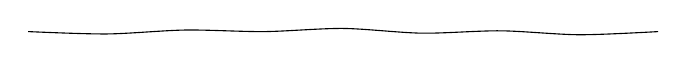
\begin{tikzpicture}\draw plot[smooth] coordinates {(0,0) (1,-.03) (2,.02) (3,0) (4,.04) (5,-.02) (6,.01) (7,-.04) (8,0)};\end{tikzpicture}}
\mspage{12}
